\documentclass{article}

% AlpaSim technical report (nuPlan track), team amanupg. Built on the organisers' template
% (neurips_2026.sty and README.md in this folder); not a NeurIPS submission.
% DRAFT 2026-11-14 for the final entry. Assumes v10 = plain W1 (released waypoints posttrain seed 1).
% Red TODOs need Aman's input, the official v10 result, or the last DAgger numbers. Not uploaded anywhere.
\PassOptionsToPackage{numbers}{natbib}
\usepackage[preprint]{neurips_2026}
\makeatletter
\renewcommand{\@noticestring}{}
\makeatother

\usepackage[utf8]{inputenc}
\usepackage[T1]{fontenc}
\usepackage{hyperref}
\usepackage{booktabs}
\usepackage{xcolor}
\usepackage{amsmath}
\usepackage{tikz}
\usetikzlibrary{positioning,arrows.meta}

\newcommand{\todo}[1]{\textcolor{red}{[TODO: #1]}}

\title{Local Gains That Did Not Transfer: Closed-Loop Lessons From Adapting a Released Latent TransFuser\\
\large AlpaSim E2E Closed Loop Challenge Technical Report (nuPlan track)}

\author{
  Team amanupg \\
  \todo{author name(s), organization} \\
  \texttt{\todo{contact email}}
}

\begin{document}
\maketitle

\begin{abstract}
Our final nuPlan entry is the released py123d\_garage v0.2.0 latent TransFuser (waypoints head, post-trained,
seed 1), run unmodified. We submit it because nothing we built beat it under a test we trust. This report is about
that test. Over the challenge we tried a learned critic, two start-from-rest rules, ensembles, speed caps,
controller gains, nuPlan fine-tuning with weight averaging, and on-policy distillation (DAgger) through the
planner's exact inference path. Three entries that improved local nuPlan scores with confidence intervals above zero
(+0.012 to +0.128 mean scene score, on up to 754 paired scenes including held-out ones) all lost on the board, by
225 to 288 PCS for the two rule add-ons. A second local benchmark, NuRec reconstructions with longer scenes,
predicted the board's direction in 3 of 3 cases where local nuPlan predicted 0 of 3. We describe the diagnosis
behind the rules (the policy plans ``wait, then go'' at every replan from rest), why it did not transfer, a
cheap board-side control (other teams' unmodified baselines), and a sampler-exact DAgger objective.
\todo{official v10 result: PCS, mean, km per at-fault incident.}
\end{abstract}

\section{Final policy}
\textbf{Model.} The released py123d\_garage~\cite{py123d} \texttt{ltf-base-waypoints-68M}, post-train stage,
seed 1 (\texttt{model\_1.pth}, 67.1M parameters, loaded strictly). It is a camera-only latent TransFuser: a
latent BEV query replaces LiDAR. On nuPlan it sees the front camera at the current frame and 1\,s earlier, the
ego state, and up to three route target points 40, 60 and 80\,m ahead. A flow-matching planning decoder outputs 64
waypoints over 6.4\,s. At inference the decoder integrates its velocity field with 8 Euler steps starting from the
zero state (noise temperature 0, one sample), so the served plan is deterministic. The simulator's MPC controller
tracks the plan, and the policy replans every 0.5\,s (Fig.~\ref{fig:system}). This is the checkpoint behind the
organisers' own board entry \texttt{093-nuplan-v1}. Our harness reproduces their published per-scene results
(182 of 200 scenes identical, mean difference $-0.0000$).

\begin{figure}[h]
\centering
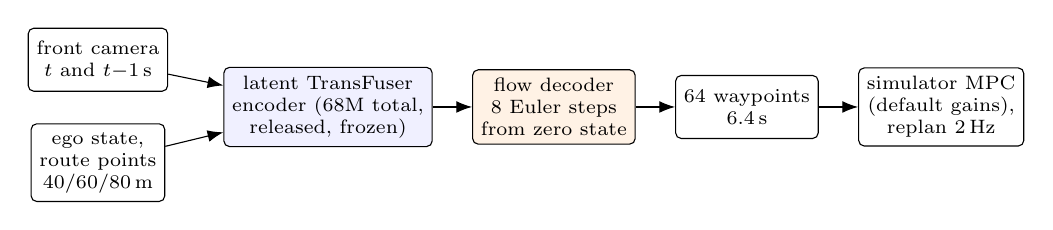
\begin{tikzpicture}[node distance=4mm and 5mm, font=\scriptsize,
  box/.style={draw, rounded corners=2pt, align=center, minimum height=8mm, inner sep=3pt},
  ar/.style={-{Latex[length=2mm]}}]
\node[box] (cam) {front camera\\$t$ and $t{-}1$\,s};
\node[box, below=of cam] (ego) {ego state,\\route points\\40/60/80\,m};
\node[box, right=7mm of cam, yshift=-6mm, fill=blue!6] (enc) {latent TransFuser\\encoder (68M total,\\released, frozen)};
\node[box, right=of enc, fill=orange!10] (dec) {flow decoder\\8 Euler steps\\from zero state};
\node[box, right=of dec] (plan) {64 waypoints\\6.4\,s};
\node[box, right=of plan] (mpc) {simulator MPC\\(default gains),\\replan 2\,Hz};
\draw[ar] (cam) -- (enc); \draw[ar] (ego) -- (enc); \draw[ar] (enc) -- (dec); \draw[ar] (dec) -- (plan);
\draw[ar] (plan) -- (mpc);
\end{tikzpicture}
\caption{Final entry: the released model, unmodified. Our DAgger experiments (Sec.~\ref{sec:dagger})
fine-tuned only the orange decoder.}
\label{fig:system}
\end{figure}

\section{Resources, training and runtime}
\textbf{Weights:} \texttt{v0.2.0/ltf-base-waypoints-68M/posttrain/model\_1.pth} with its \texttt{config.yaml} and
\texttt{sensor\_rig\_nuplan.yaml}, Hugging Face \texttt{kesai-labs/py123d\_garage\_pretrained\_checkpoints} at
revision \texttt{56edbe90}, released under Apache-2.0 at that revision (the repository was relicensed to
CC BY-NC-SA 4.0 on 2026-10-29). KE:SAI trained it on public data: Physical AI AV, NuRec and nuPlan train/val.
\textbf{Code:} py123d\_garage v0.2.2 (Apache-2.0) and \texttt{alpasim\_grpc} 0.54.0 from NVlabs/alpasim
\texttt{e2e\_challenge} (Apache-2.0). \textbf{Training:} none for the final entry. \textbf{Runtime:} the official
v9 run of the same model plus a rule add-on took 1,235\,s of the 3,000\,s budget for 1,000 rollouts.
\todo{v10 wall time and GPU memory.} The image is offline with all weights included.

Our experiments additionally used the public nuPlan navtest assets (\texttt{OpenDriveLab/AlpasimChallenge2026\_nuplan\_track})
and NuRec scenes for local closed-loop evaluation, and nuPlan logs for one fine-tune. No private-set data,
per-scene private results, or other teams' weights were used for any choice.

\section{Evaluation protocol}
\textbf{Local nuPlan.} The simulator is deterministic on one GPU type, so we compared policies per scene on the
same scenes, with 90\% bootstrap intervals. A change counted as a gain only if positive on tuning (300 scenes),
held-out (261) and fresh scenes (193 to 691) with the interval above zero and no new at-fault collisions.
\textbf{NuRec.} 440 reconstructed scenes, about 20\,s each with many mid-scene stops (nuPlan scenes are about 5\,s).
\textbf{Board controls.} Four other teams submitted the released joint64 seed 0 checkpoint unchanged and scored
the same mean scene score (0.9205) and PCS within 10 points of each other. Comparing an add-on to these entries isolates
its effect on the private set without spending a slot.

\section{What we tried and what the board said}
\begin{table}[h]
\centering\footnotesize\setlength{\tabcolsep}{3pt}
\begin{tabular}{lccc}
\toprule
Entry (change) & local nuPlan gain [90\%] & NuRec & board vs its base \\
\midrule
v6: critic substitution + stall rescue & +0.128 [+0.108, +0.149] (754) & -- & 0.782 vs 0.848 mean \\
v8: start-now from rest, joint64 s0 & +0.012 (754, CI $>0$ per group) & flat, +3 at-fault & $-0.012$ mean, $\approx-225$ PCS \\
v9: drop-the-wait nudge, W1 & +0.012 (600 fresh, 0 losses) & +4/$-1$ at-fault & $-0.018$ mean, $\approx-288$ PCS \\
\bottomrule
\end{tabular}
\caption{Every submitted change gained locally on nuPlan and lost on the board. The NuRec column showed more at-fault
incidents for both rule add-ons, matching the board. ``Board vs its base'' compares v8 with the four unmodified
joint64 seed 0 entries and v9 with the organisers' W1 entry.}
\label{tab:board}
\end{table}

\textbf{Start-from-rest diagnosis.} Plan logs show that from rest the released policy plans ``wait about 2\,s, then
go'' at every replan. Because it replans every 0.5\,s, the start keeps moving away, and the ego never starts.
Dropping the waiting prefix after $K=3$ such plans (v8), or only when the model's own detections show a clear
corridor (v9), fixed stuck scenes locally with no new failures in 600 to 754 scenes. On the board both lowered the
distance per at-fault incident (W1 0.981 to 0.712\,km for v9). NuRec showed why: with longer scenes the rule fires
about 8 times more often, and the extra incidents were front collisions about 2\,s after the release (a left turn
into an oncoming car, a merging car). Waiting was right in those cases. The private set is cut from about 20 log
segments into overlapping starts, so one such situation can zero 5 to 15 scenes, which matches the size of the
losses.

\textbf{Checks that also failed} (paired, fresh nuPlan unless noted). 3-seed plan ensemble: NuRec $-0.023$,
W25/L57 (147 scenes). Speed cap at 0.9 of the planned speed: $-0.013$, W2/L89 (500). Turn-only cap (0.8 above
15$^\circ$): $+0.000$ on both benchmarks; a binding cap (0.6 above 10$^\circ$) cut NuRec at-fault incidents 61 to
52 but cost progress ($-0.008$ nuPlan, $-0.004$ NuRec). Controller heading weight 2.0: $-0.005$, 2 new zero
scenes; steering-rate weight 2.5: $-0.003$, 1 new zero scene. nuPlan-only fine-tune of v0.2.0 (tuning scenes): $-0.012$, and
weight averaging with the base: $\pm0.001$. Replan rate is a no-op on nuPlan (control step fixed at 0.5\,s). A local
PCS proxy built with the organisers' IRT code ranked v8 above its base even with the host's 12 checkpoints in the
population, the opposite of the board.

\section{Sampler-exact on-policy distillation}
\label{sec:dagger}
\textbf{Objective.} The released flow-matching loss trains the decoder on paths from random noise, but the served
plan is the 8-step Euler integral from the zero state, a path the training loss never visits. We train through the
served plan itself: unroll the 8 steps differentiably and apply a masked L1 loss (positions and yaw) between that
plan and the label. A check confirmed the unrolled plan equals the sampled one (0.000\,m) and the recorded one
(0.010\,m, GPU-type rounding). Only the decoder is trained (14.9M of 67.1M parameters), and the whole policy stays
in eval mode so frozen normalisation statistics do not drift.

\textbf{Data.} W1 drives 319 local training scenes that share no log with the 691 evaluation scenes. Runs are clean
or with exploration noise on the served plan (probability 0.5, lateral offset up to 0.8\,m ramped over 2\,s, speed
scaled by 0.8 to 1.2). Each reached state is labelled with the human's logged future, blended back from the current
pose over 2\,s (recording ground truth is a local simulator switch; the submission never sees it). Variants:
human labels everywhere (D1), or human labels only where the ego is at least 1\,m (D1o, D2o) or 0.5\,m (D2h) off the
human path and the model's own plan elsewhere. We also tested reward-filtered self-imitation (keep the
best-scoring noisy rollout per scene): noise improved only 1 of 79 scenes and fixed none of W1's failures, so it had
no signal to train on.

\textbf{Results} (paired vs W1, 100 fresh scenes per part). D1: $-0.059$, $+0.021$, $-0.059$, $-0.097$,
$-0.044$ on five parts (overfit after one epoch on 79 scenes). D1o: $-0.017$, $-0.002$, $+0.002$ on three parts.
\todo{D1o remaining parts, D2o and D2h on 691 scenes; NuRec if any passes.} Imitating human recovery labels moved
the planner away from the released behaviour faster than it fixed failures.

\section{Limitations and safety}
The entry inherits W1's behaviour and failure modes. Locally its remaining zero scores are mostly off-road exits from
sub-metre lateral drift that the predicted BEV map cannot resolve, plus slow starts from rest. For the
related joint64 checkpoint, 5 of its 22 local zero-score scenes also failed when the ego replayed the log, so some
failures are unavoidable. We changed nothing that
affects safety. Our main lesson is about validation: a rule that only fires in rare situations can pass hundreds of
local scenes and still fail on a private set built from a few logs. Tests with longer scenes (NuRec) and
board-side controls caught this; scene-level confidence intervals on short local scenes did not.

\begin{thebibliography}{9}
\bibitem{py123d} KE:SAI. \newblock py123d\_garage: training and closed-loop evaluation framework with pretrained
  baselines for the AlpaSim E2E Challenge. \newblock \url{https://github.com/kesai-labs/py123d_garage}, 2026.
\bibitem{nuplan} H.~Caesar et al. \newblock nuPlan: A closed-loop ML-based planning benchmark for autonomous vehicles.
  \newblock arXiv:2106.11810, 2021.
\bibitem{alpasim} NVIDIA. \newblock AlpaSim. \newblock \url{https://github.com/NVlabs/alpasim}, 2026.
\end{thebibliography}

\end{document}
